\documentclass{standalone}

\usepackage{tikz}
\usetikzlibrary{arrows}
\usetikzlibrary{decorations.markings}
\usetikzlibrary{calc}

\begin{document}

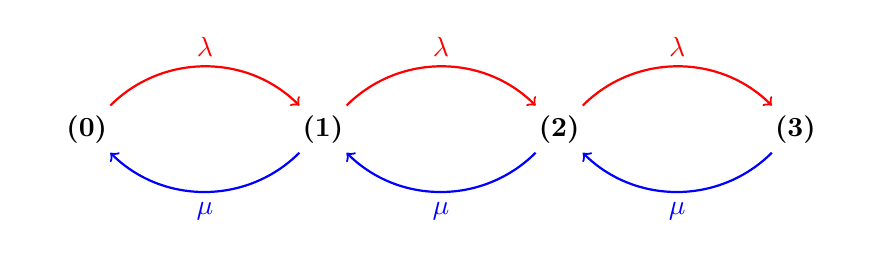
\begin{tikzpicture}
    \tikzstyle{state}=[minimum width=1.5cm, font=\boldmath];

    \node (0) at (0,0) [state] {$(0)$};
    \node (1) at ($(0)+(3,0)$) [state] {$(1)$};
    \node (2) at ($(1)+(3,0)$) [state] {$(2)$};
    \node (3) at ($(2)+(3,0)$) [state] {$(3)$};


    % Transitions
    % Arrivals

    \draw[draw=red] (0) edge[out=45,in=135,->,thick] node [above, text=red] {$\lambda$}  (1);
    \draw[draw=red] (1) edge[out=45,in=135,->,thick] node [above, text=red] {$\lambda$}  (2);
    \draw[draw=red] (2) edge[out=45,in=135,->,thick] node [above, text=red] {$\lambda$}  (3);

    % Services

    \draw[draw=blue] (0) edge[out=-45,in=-135,<-,thick] node [below, text=blue] {$\mu$} (1);
    \draw[draw=blue] (1) edge[out=-45,in=-135,<-,thick] node [below, text=blue] {$\mu$} (2);
    \draw[draw=blue] (2) edge[out=-45,in=-135,<-,thick] node [below, text=blue] {$\mu$} (3);


\end{tikzpicture}

\end{document}
